\chapter{WIFI Module}

\section{Description}

Portenta H7 comes with an on-board Wi-Fi  Module that allows to develop IoT applications that require wireless connectivity and Internet access. Turning the board into an access point allows to create a Wi-Fi network on its own and allows other devices to connect to it. \cite{portentaWifiAccessPoint:2024}
\newline

\textbf{Key Features:}
\begin{itemize}
	
	\item \textbf{Dual-Band WiFi Connectivity:} The Portenta H7 supports both 2.4 GHz and 5 GHz WiFi bands, ensuring a reliable and fast connection in various network environments, whether in congested areas or high-speed applications. 
	
	\item \textbf{Robust Security:} Equipped with WPA3 support, the WiFi module on the Portenta H7 provides cutting-edge security features, ensuring that data transmission is secure and protected from unauthorized access. 
	
	\item \textbf{Seamless IoT Integration:} The WiFi module allows for easy integration into cloud platforms and IoT applications, enabling seamless data collection, remote monitoring, and real-time communication in connected systems. 
	
	\item \textbf{High Throughput:} Capable of high data transfer rates, the WiFi module can handle large volumes of data, making it ideal for applications such as real-time video streaming, telemetry, or large-scale sensor networks. 
	
	\item \textbf{Energy Efficient:} Designed to support low-power modes, the WiFi module can maintain wireless connectivity while conserving energy, ideal for battery-operated devices and power-conscious applications. \cite{portentaWifiAccessPoint:2024}
	
\end{itemize}

\section{Specific Sensor}
The WiFi functionality in the Portenta H7 is powered by an integrated module that adheres to the 802.11 standards, supporting both 2.4 GHz and 5 GHz frequency bands. This module enables seamless wireless communication, offering high data throughput and robust performance in a variety of network conditions.
\newline
The onboard WiFi/Bluetooth module provides the Portenta H7 with the capability to connect wirelessly to local networks, cloud services, and IoT platforms. The dual-band WiFi support allows the board to connect to a wide range of network environments, optimizing both speed and stability. \cite{portentaWifiAccessPoint:2024}

\section{Specification}

\begin{itemize}
	
	\item The WiFi module on the Arduino Portenta H7 supports the IEEE 802.11 a/b/g/n standards.
	\item It offers dual-band connectivity (2.4 GHz and 5 GHz) for flexible network compatibility.
	\item The WiFi module can achieve data transfer rates up to 150 Mbps, suitable for demanding applications such as real-time data streaming and cloud communication.
	\item It supports WPA3 encryption, ensuring secure communication across networks.
	\item The WiFi module operates with low power consumption, making it ideal for IoT applications and battery-powered projects.
	\item The WiFi module can be programmed using the Arduino IDE with the WiFi libraries available for the Portenta H7. \cite{portentaWifiAccessPoint:2024}
	
\end{itemize}

\section{TESTS}

\subsection{WiFi Access Point}
The onboard Bluetooth module of the Portenta H7 offers low energy Bluetooth functionality, in order to provide the board with the flexibility to be easily connected to devices which also support Bluetooth Low Energy, such as the Arduino Nano 33 IoT or most modern smartphones. Compared to classic Bluetooth, Low Energy Bluetooth is intended to provide considerably reduced power consumption and cost while maintaining a similar communication range. \cite{portentaWifiAccessPoint:2024} 

\subsubsection{Overview}
Portenta H7 comes with an on-board Wi-Fi and a Bluetooth Module that allows to develop IoT applications that require wireless connectivity and Internet access. Turning the board into an access point allows to create a Wi-Fi network on its own and allows other devices to connect to it. In this tutorial you will learn to set up your board as an access point web server and remotely control the red, green and blue LEDs on the built-in RGB LED by accessing an HTML page on your mobile device’s browser. \cite{portentaWifiAccessPoint:2024}

\subsubsection{Goals}
\begin{itemize}
	\item About the built-in Wi-Fi + Bluetooth module.
	\item How a client-server model works. \cite{portentaWifiAccessPoint:2024}
	\item How to create an HTTP communication channel between the board and an external device. \cite{portentaWifiAccessPoint:2024}
\end{itemize}

\subsubsection {Required Hardware and Software}
\begin{enumerate}
	\item Portenta H7 or Portenta H7 Lite Connected 
	\item USB-C cable (either USB-A to USB-C)
	\item Arduino IDE 1.8.13+ or Arduino Pro IDE 0.0.4+
	\item A smart phone \cite{portentaWifiAccessPoint:2024}
\end{enumerate}

\textbf{Access Point Configuration}  \newline

The Portenta H7 features a Murata 1DX, which is a high performance chipset which supports Wi-Fi 802.11b/g/n + Bluetooth 5.1 BR/EDR/LE, up to 65 Mbps PHY data rate on Wi-Fi and 3 Mbps PHY data rate on Bluetooth. This module helps to configure the Portenta into three different modes of operation - an Access Point, a Station, or both. In this tutorial we will only focus on the access point configuration.

When the board is configured to operate as an access point, it can create its own wireless LAN (WLAN) network. In this mode, the board transmits and receives signals at 2.4 GHz allowing other electronic devices with Wi-Fi capabilities using the same bandwidth to connect to the board.

\begin{figure}
	\begin{center}
		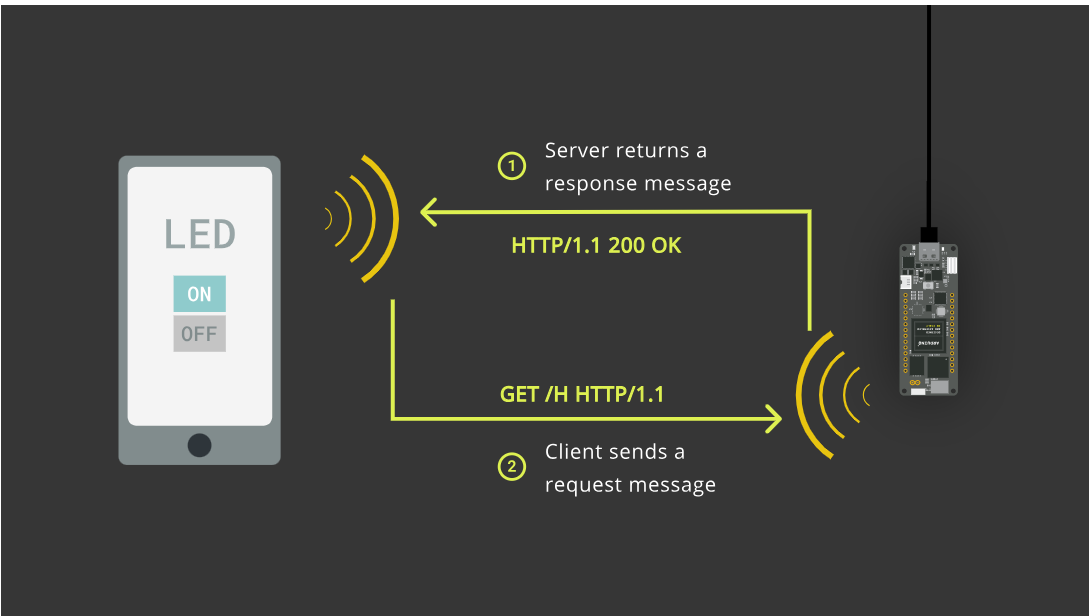
\includegraphics[width=0.7\linewidth]{Images/WIFI Module/Full Interface.png}
		\caption{Full Interface}
		\label{Full Interface} \cite{portentaWifiAccessPoint:2024}
	\end{center}
\end{figure}

With the access point set up, you create a client server architecture where the board provides a web server communicating with the client devices over HTTP. The connected devices can then make HTTP GET requests to the server to retrieve web pages served by the web server on the board. This makes the Portenta H7 an ideal board for developing IoT solutions where external client devices can send and receive information while more complex processing tasks take place on the server. \cite{portentaWifiAccessPoint:2024}

\subsubsection{Instructions}

\begin{itemize}
	\item \textbf{Setting Up the Web Server:} In this tutorial you are going to convert the board into an access point and use it to set up a web server which provides a HTML webpage. This page contains buttons to toggle the red, green and blue color of the built-in LED. You will then connect your mobile device to this access point and access this web page through the browser on your mobile phone. Once retrieved, you will be able to control the state of the red, green and blue LED on the built-in RGB LED from your mobile device. ~\ref{SetUpServer} \cite{portentaWifiAccessPoint:2024}
	
	\begin{figure}
		\begin{center}
			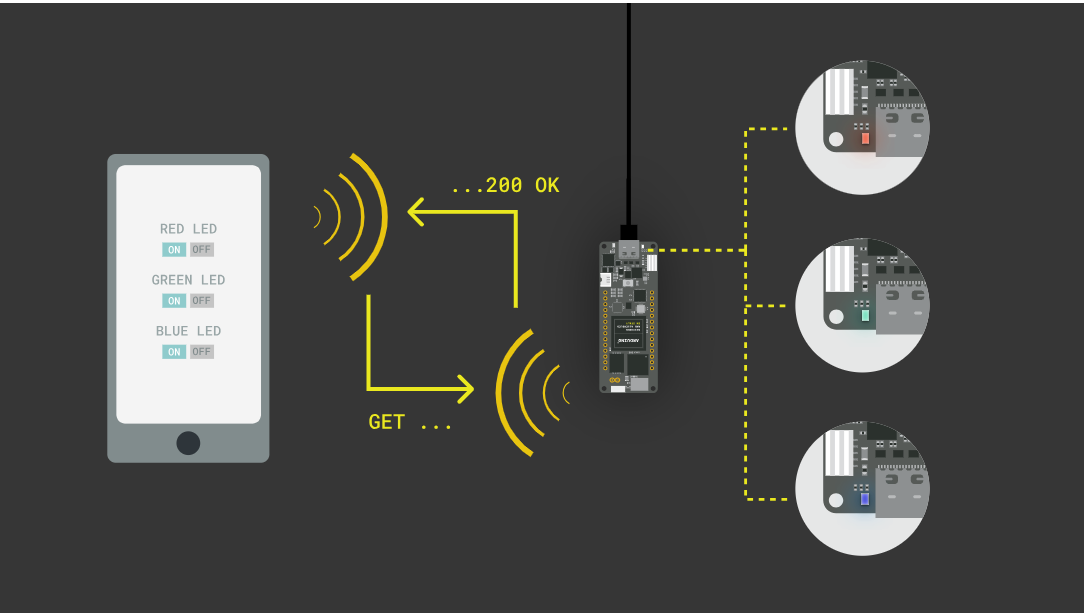
\includegraphics[width=0.7\linewidth]{Images/WIFI Module/SetUpServer.png}
			\caption{SetUpServer}
			\label{SetUpServer} \cite{portentaWifiAccessPoint:2024}
		\end{center}
	\end{figure}
	
	\item \textbf{1. The Basic Setup:} Begin by plugging in your Portenta board to your computer using a USB-C cable and open the Arduino IDE. If this is your first time running Arduino sketch files on the board, we suggest you check out how to set up the Portenta H7 for Arduino before you proceed. ~\ref{The Portenta H7 can be connected to the computer using an appropriate USB-C cable} \cite{portentaWifiAccessPoint:2024}
	
	\begin{figure}
		\begin{center}
			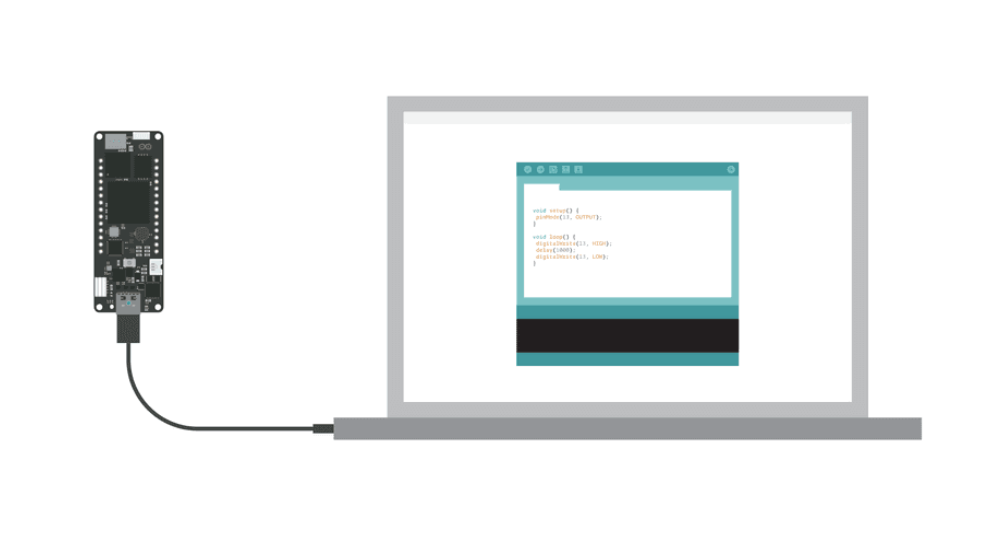
\includegraphics[width=0.7\linewidth]{Images/WIFI Module/BasicSetup.png}
			\caption{BasicSetup}
			\label{The Portenta H7 can be connected to the computer using an appropriate USB-C cable} \cite{portentaWifiAccessPoint:2024}
		\end{center}
	\end{figure}
	
	\item \textbf{2. Create the Web Server Sketch:} Next you need to create a web server sketch that will handle the HTTP GET requests and provide the client devices with the HTML web page. The Wi-Fi library provides all necessary methods that allows Arduino boards to use their Wi-Fi features provided by the on-board Wi-Fi module. To set up the web server copy the following code, paste it into a new sketch file and name it \SHELL{SimpleWebServer.ino}. ~\ref{LEDState} \cite{portentaWifiAccessPoint:2024}
	

	\begin{figure}
		\begin{center}
			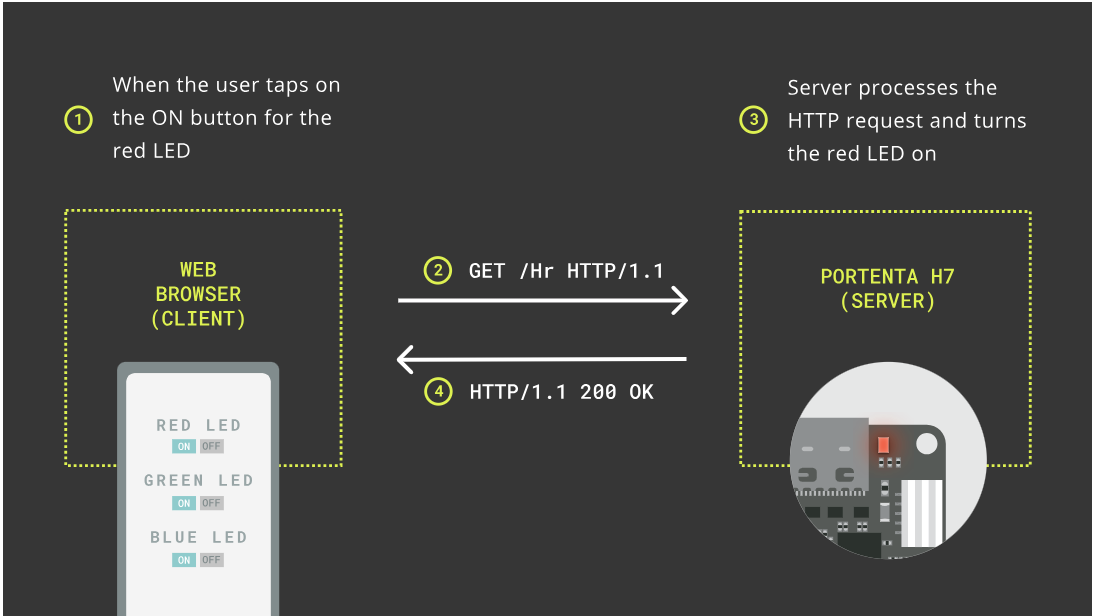
\includegraphics[width=0.7\linewidth]{Images/WIFI Module/LEDState.png}
			\caption{LEDState}
			\label{LEDState} \cite{portentaWifiAccessPoint:2024}
		\end{center}
	\end{figure}

	{
		\captionof{code}{Simple sketch to control the LED using bluetooth}\label{PortentaBLE}
		\ArduinoExternal{}{../Code/Wifi/SimpleWebServer/SimpleWebServer.ino}
	}
	
	This sketch describes how the server will handle an incoming HTTP GET request from a client, both to request the HTML web page from the server and the requests to change the LED states using dedicated URLs.
	
	Here the web page is just a simple HTML page with buttons to toggle the LED states. The way in which the web page works is: whenever a button on the web page is pressed, the client device (in this case your phone) sends a HTTP GET request to a URL denoted by a letter, in this case H or L (H stands for HIGH, L stands for LOW) followed by the LED color that should be turned on or off r, g or b. For example, to turn on the red LED the URL is /Hr . Once the server receives this request, it changes the corresponding LED state, closes the connection and continues to listen to next requests. \cite{portentaWifiAccessPoint:2024}
	
	
	
	
	\item \textbf{3. Create the arduino secrets.h Tab:} A good practice is to have sensitive data like the SSID and the password required to identify and connect to a certain network within a separate file. Click on the arrow icon below the Serial Monitor button and open a new tab in the Arduino IDE. This will create a new file.. ~\ref{PortentaBLE} \cite{portentaWifiAccessPoint:2024}
	
	\begin{figure}
		\begin{center}
			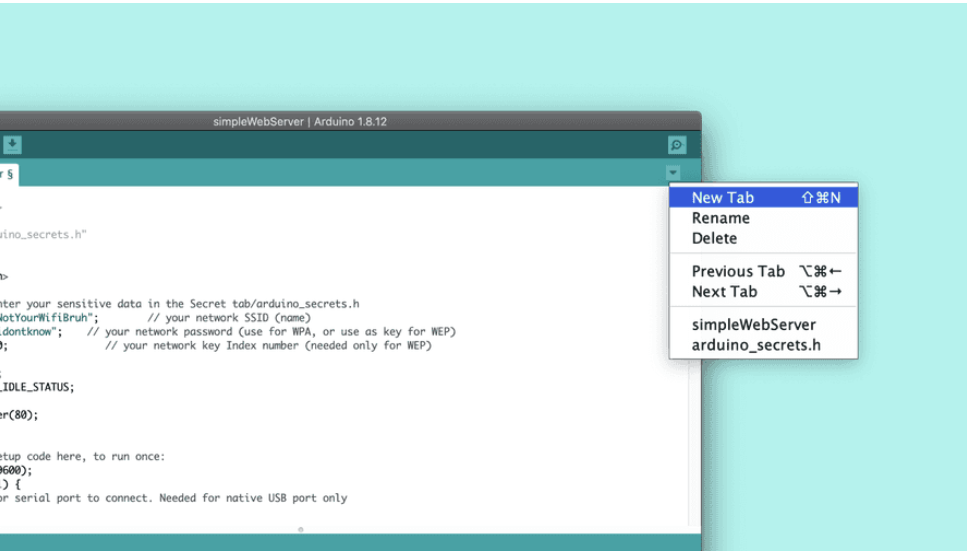
\includegraphics[width=0.7\linewidth]{Images/WIFI Module/NewTab.png}
			\caption{NewTab}
			\label{NewTab} \cite{portentaWifiAccessPoint:2024}
		\end{center}
	\end{figure}
	
	Name the file \SHELL{arduino secrets.h} and click OK.
	
	\begin{figure}
		\begin{center}
			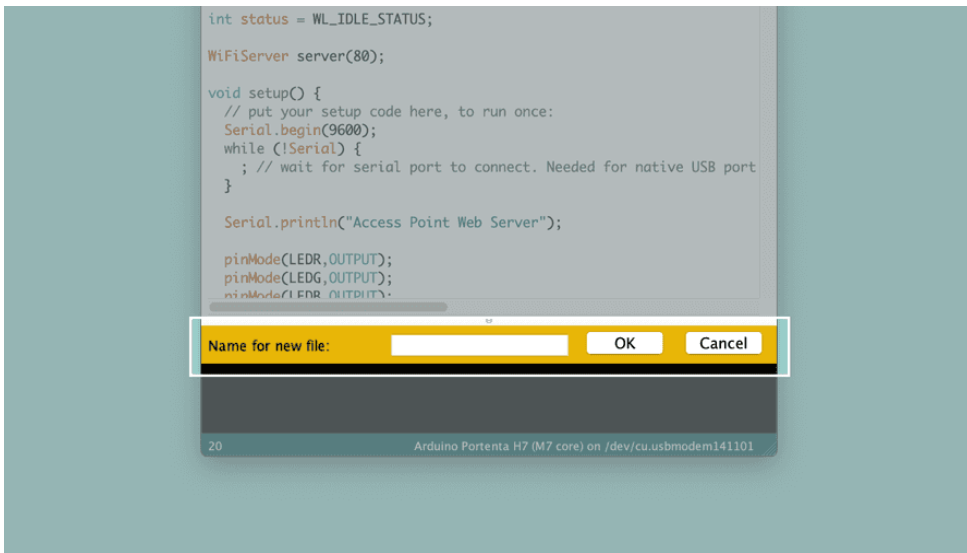
\includegraphics[width=0.7\linewidth]{Images/WIFI Module/NamingNewTab.png}
			\caption{NamingNewTab}
			\label{NamingNewTab} \cite{portentaWifiAccessPoint:2024}
		\end{center}
	\end{figure}
	
	Once you have created the new tab, you will see an empty page in the IDE. Define two constants \SHELL{SECRET SSID} and \SHELL{SECRET PASS} that will hold the name of the Wi-Fi network and the corresponding password. Add the following lines to your \SHELL{arduino secrets.h} file:
	
	\begin{lstlisting}[language=C++, frame=single, numbers=left, basicstyle=\ttfamily\small]
		# define SECRET SSID "PortentaAccessPoint"
		# define SECRET PASS "123Qwerty"
	\end{lstlisting}
	
	In order to access the \SHELL{SECRET SSID} and \SHELL{SECRET PASS} constants in the \SHELL{simpleWebServer.ino} sketch file, the header file that you have just created needs to be included. In your sketch file this has already been taken care of by the following line at the beginning of the sketch:
	
	\begin{lstlisting}[language=C++, frame=single, numbers=left, basicstyle=\ttfamily\small]
		#include "arduino_secrets.h"
	\end{lstlisting}
	
	\begin{figure}
		\begin{center}
			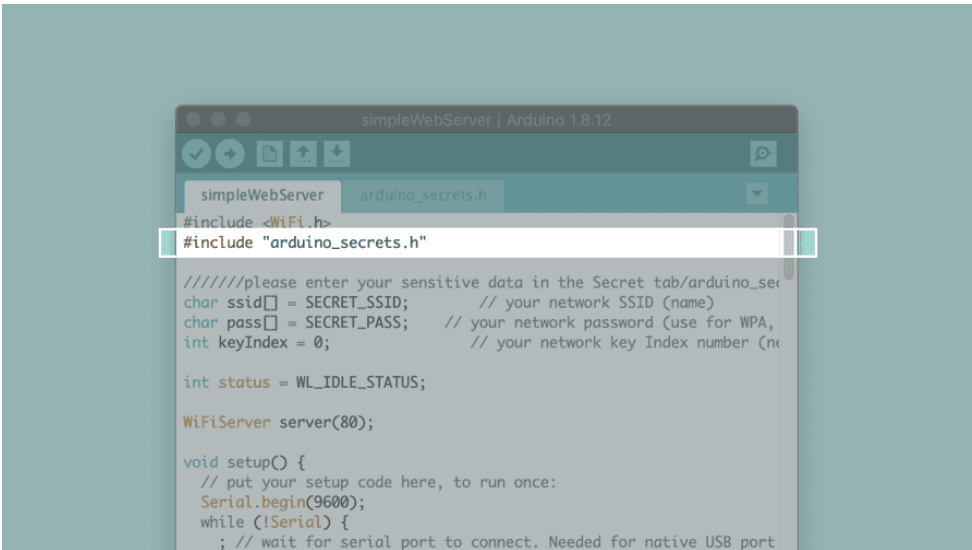
\includegraphics[width=0.7\linewidth]{Images/WIFI Module/HeaderFile.png}
			\caption{HeaderFile}
			\label{HeaderFile} \cite{portentaWifiAccessPoint:2024}
		\end{center}
	\end{figure}
	
	
	\item \textbf{4. Upload the Code:}Select the Arduino Portenta H7 (M7 core) from the Board menu and the port the Portenta is connected to. Upload the simpleWebServer.ino sketch. Doing so will automatically compile the sketch beforehand. ~\ref{Uplaoding}
	
	\begin{figure}
		\begin{center}
			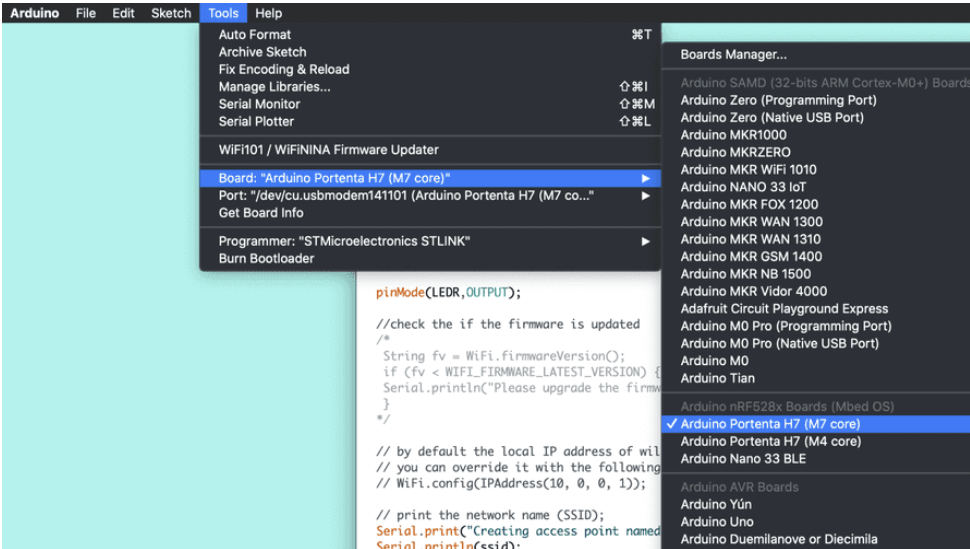
\includegraphics[width=0.7\linewidth]{Images/WIFI Module/Uplaoding.png}
			\caption{Uplaoding}
			\label{Uplaoding} \cite{portentaWifiAccessPoint:2024}
		\end{center}
	\end{figure}
	
	Once you have uploaded the code, open the Serial Monitor. You will be able to see the IP address of the access point. You will also see the message, Device disconnected from AP which means there are no devices connected to the Access point yet.
	
	\begin{figure}
		\begin{center}
			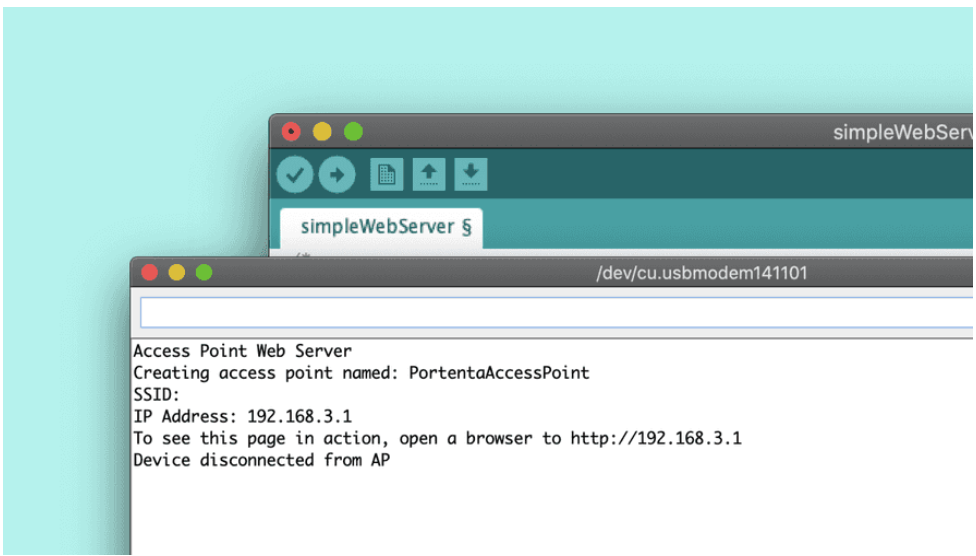
\includegraphics[width=0.7\linewidth]{Images/WIFI Module/SerialMonitor.png}
			\caption{SerialMonitor}
			\label{SerialMonitor} \cite{portentaWifiAccessPoint:2024}
		\end{center}
	\end{figure}
	
	
	\item \textbf{5. Connecting to the Portenta Access Point:} Once the access point is active and ready to be connected with external devices, you will be able to find the PortentaAccessPoint on the list of networks on your mobile device. Once you have entered the password you have defined earlier, your smart phone will connect to access point.. ~\ref{PortentaAccessPoint}	 \cite{portentaWifiAccessPoint:2024}
	
	\begin{figure}
		\begin{center}
			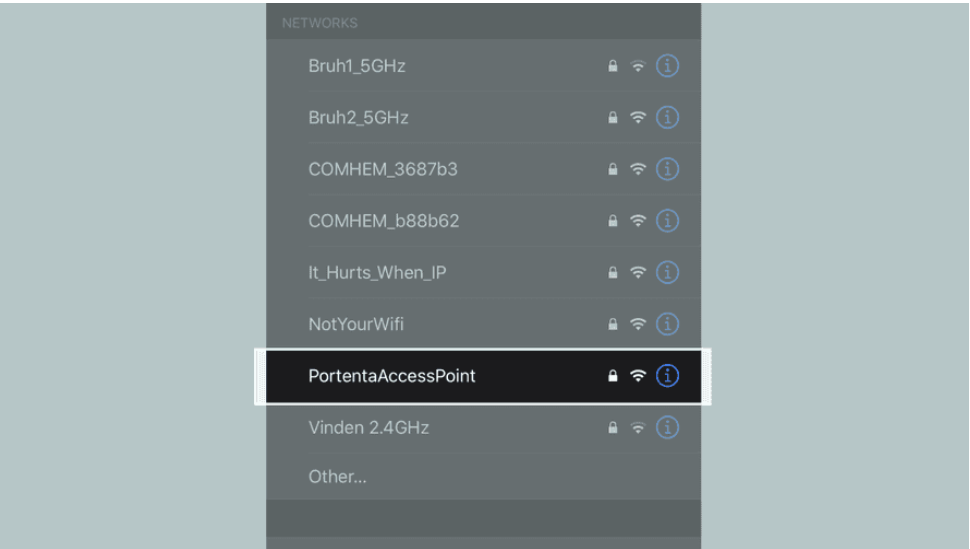
\includegraphics[width=0.7\linewidth]{Images/WIFI Module/PortentaAccessPoint.png}
			\caption{PortentaAccessPoint}
			\label{PortentaAccessPoint} \cite{portentaWifiAccessPoint:2024}
		\end{center}
	\end{figure}
	
	Now open a browser window on your mobile device and copy and paste the URL containing Portenta’s IP address that is displayed on the serial monitor.
	
	\begin{figure}
		\begin{center}
			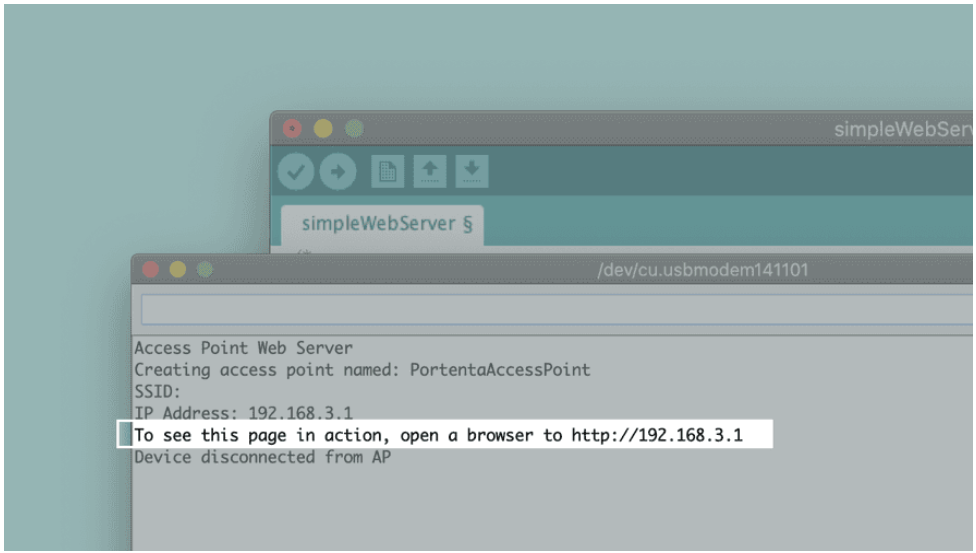
\includegraphics[width=0.7\linewidth]{Images/WIFI Module/URLAccessPoint.png}
			\caption{URLAccessPoint}
			\label{URLAccessPoint} \cite{portentaWifiAccessPoint:2024}
		\end{center}
	\end{figure}
	
	Once you have entered the URL, the client sends a GET request to the web server to fetch the HTML web page specified in the code. Once loaded, you will see the web page in your mobile browser.
	
	\begin{figure}
		\begin{center}
			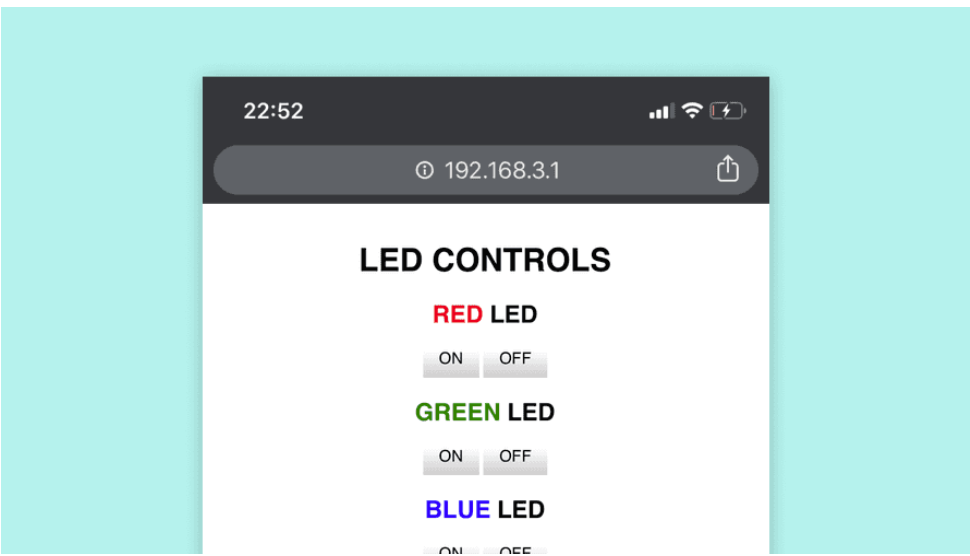
\includegraphics[width=0.7\linewidth]{Images/WIFI Module/HTML Page.png}
			\caption{HTML Page}
			\label{HTML Page} \cite{portentaWifiAccessPoint:2024}
		\end{center}
	\end{figure}
	
	\item \textbf{5. Access the Board From Your Mobile Device:} If you take a look at the Serial Monitor, you can see the details of the HTTP GET request and other details of the device connected to the access point. The GET request is always in the following format:.	 \cite{portentaWifiAccessPoint:2024}
	
	\begin{lstlisting}[language=C++, frame=single, numbers=left, basicstyle=\ttfamily\small]
		GET URL HTTP/1.1
	\end{lstlisting}
	
	The URL is a string of characters sent to the server, in this case /Hx (where x stands for the color of the LED). This request containing the URL is received on the server and it replies with the following HTTP/1.1 response indicating that the connection was successful:
	
	\begin{lstlisting}[language=C++, frame=single, numbers=left, basicstyle=\ttfamily\small]
		HTTP/1.1 200 OK
	\end{lstlisting}
	
	Once the server has responded to this request, it closes the connection and continues listening to next GET requests.
	
	\begin{figure}
		\begin{center}
			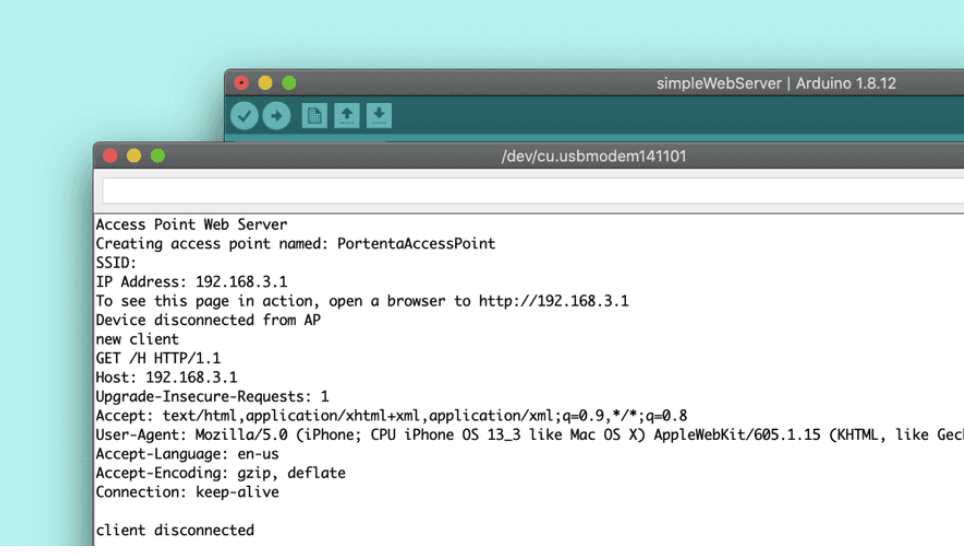
\includegraphics[width=0.7\linewidth]{Images/WIFI Module/ClientDetails.png}
			\caption{ClientDetails}
			\label{ClientDetails} \cite{portentaWifiAccessPoint:2024}
		\end{center}
	\end{figure}
	
	You are now be able to toggle the states of the red, green and blue LED through the buttons displayed on your mobile browser. Every time you press a button, the client sends a GET request to a URL in the format /Hx or /Lx ,where x can be ‘r’, ‘g’ or ‘b’, depending on the button pressed on the HTML page. The web server then reads the URL requested by the client, changes the state of the LED corresponding to the URL and closes the connection. \cite{portentaWifiAccessPoint:2024}
	
	\begin{figure}
		\begin{center}
			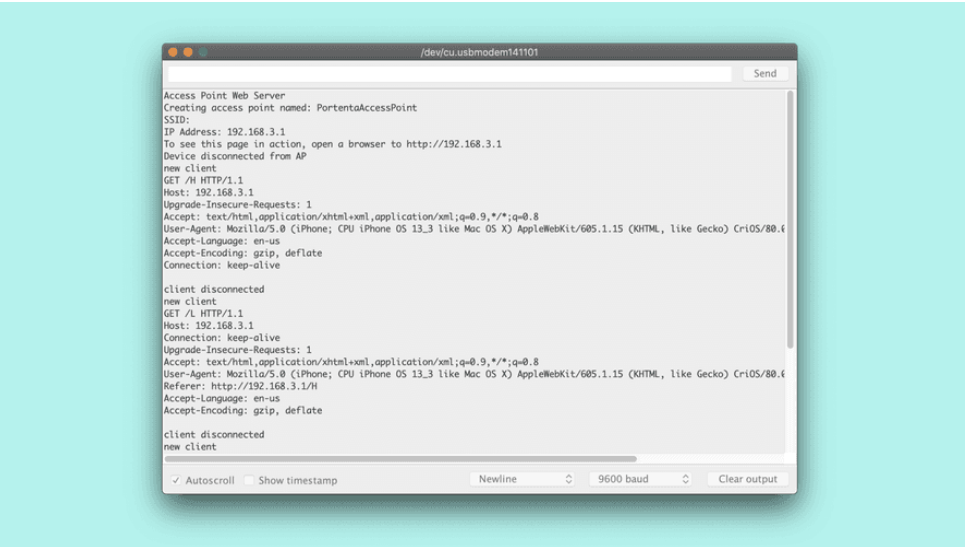
\includegraphics[width=0.7\linewidth]{Images/WIFI Module/GETRequest.png}
			\caption{GETRequest}
			\label{GETRequest} \cite{portentaWifiAccessPoint:2024}
		\end{center}
	\end{figure}
	
\end{itemize}

\subsubsection{Conclusion:}
This tutorial shows one of the several capabilities of the on-board WiFi+Bluetooth module by configuring the board as an access point and setting up a web server. You have also learnt how a simple client-server model and the underlying HTTP requests and responses work. \cite{portentaWifiAccessPoint:2024}




